%================================================
%================================================
%================================================
\chapter{Related Work}

%TODO Intro to the chapter
The general problem to study in this project is activity recognition with a mobile robot. 
In this chapter, relevant related work is reviewed.

In humans, activity recognition is a cognitive skill that can be considered mainly into perception. 
The basis to understand it relies first in Psychology, because it provides the concepts and the evidence of how the mind is constituted (\ref{ch_LitRev_Perception}). 
The next step is to look at the possibilities to mimic a cognitive process into a machine, this problem has been studied widely in Artificial Intelligence. %TODO Add cross reference
In particular, activity recognition has been studied in Computer Vision. %TODO Add cross reference
Finally, the problem has to landed to a robotic stage, making emphasis on the advantages and disadvantages of a robotic platform. %TODO Add cross ref

% 0 - GENERALITIES
% Perception
% Symbol ground
% Anchoring
% Frame Problem

\section{General antecedents - Perception in AI} \label{ch_LitRev_Perception}

Perception, as a cognitive process, has been studied widely in Psychology.
It refers to the process of organizing and interpreting sensory information so that it has a meaning \citep{King2014Psychology}.
Part of the interest is about how sensory information is processed by the brain, and which parts of it are essential.
Also relevant is the domain knowledge that the subject has about a particular context.
Together, the sensory input and the domain knowledge are used to interpret a scene.

%TODO Other interesting examples to discuss later: Plato's Cave, 5 blind men and the elephant, Flatland, Metamorfosis.

Sensory input is important for perception, however, not all the data is equally important to interpret a particular scene and conclusions can still be made, even with partial data.
In \citep{Heider1944_Experimental}, an animated film was created using only moving polygons to demonstrate how the motion of abstract entities could be interpreted by human observers in meaningful ways.
In \citep{Johansson1973_VisualPer}, locomotion patterns of living organisms using visual marks were studied. 
By this mean, the emphasis was put in the qualitative motion description of the marks rather than in the qualitative motion description of the moving body.

In Artificial Intelligence, perception has been treated mostly by the computer vision research community.
Earlier works can be traced back to the 1960s, as part of the effort to mimic human-like intelligence using visual perception components. The main difference between computer vision and image processing has been the desire to recover the three-dimensional structure of the world from images, and to use this as a stepping stone towards full scene understanding \citep{Winston1975_PsyCV}. 


One of the earlier works in 3D reconstruction from a single image is found in \citep{Roberts1963_PhDThesis}.
The developed system was able to reconstruct geometrical bodies with flat surfaces by recognizing the borders of the bodies in the scene and later analysing the shades of their visible surfaces.
%TODO Maybe include Adolfo Guzman Arenas work here. +-
In \citep{Barrow1971_RelatDesc} object recognition was studied by decomposing an image into regions and describing the spatial relations between them, in a more qualitative, rather than the traditional quantitative, approach.

Since the early 1970s, the \textit{block's world} was used as a test scenario for intelligent systems, particularly regarding knowledge representation, reasoning and planning.
In the block's world, an initial state $A$ and a desired state $B$  of the environment are given.
The goal is to autonomously generate a plan to transform $A$ into $B$ by the manipulation of the blocks.
One important characteristic of the problem is that requires a symbolic representation of the scene.
The problem was used as a test case for the robot Shakey \citep{Nilsson84_Shakey}.

%Finally, during the 1980s an approach to perception with emphasis in action feedback became popular
%TODO Complete Active Perception.

%TODO Need to mention QSR.
%TODO Need to mention KRR (ASP, DL, Ontologies, Naive Ph, etc.).


\section{Activity Recognition} 
% Emphasis in the taxomony of the area. I will only describe the taxonomy and give examples. I need to finish with describing the branch that fits better the "robotics" approach, and that will be the next section.

Activity recognition is an important research area in the context of automated perception. 
It has many applications as surveillance, inspection, verification, generation of automated reports, etc.
The application will dictate the approach to follow and the kind on sensors that will be required.

First, regarding sensing, two approaches can be followed, environmental and/or pervasive. 
The first one observes the scene from the distance as it happens with a CCTV camera or a robot. 
The pervasive approach relies on wearable devices to detect the activity of a person from a first person point of view.

Another possible classification of activity recognition systems focuses on how information is processed.
In \citep{Aggarwal11_HumanActivity} a taxonomy is proposed as shown in Fig. \ref{fig:taxonomy}.  

\begin{figure}[h]
\centering
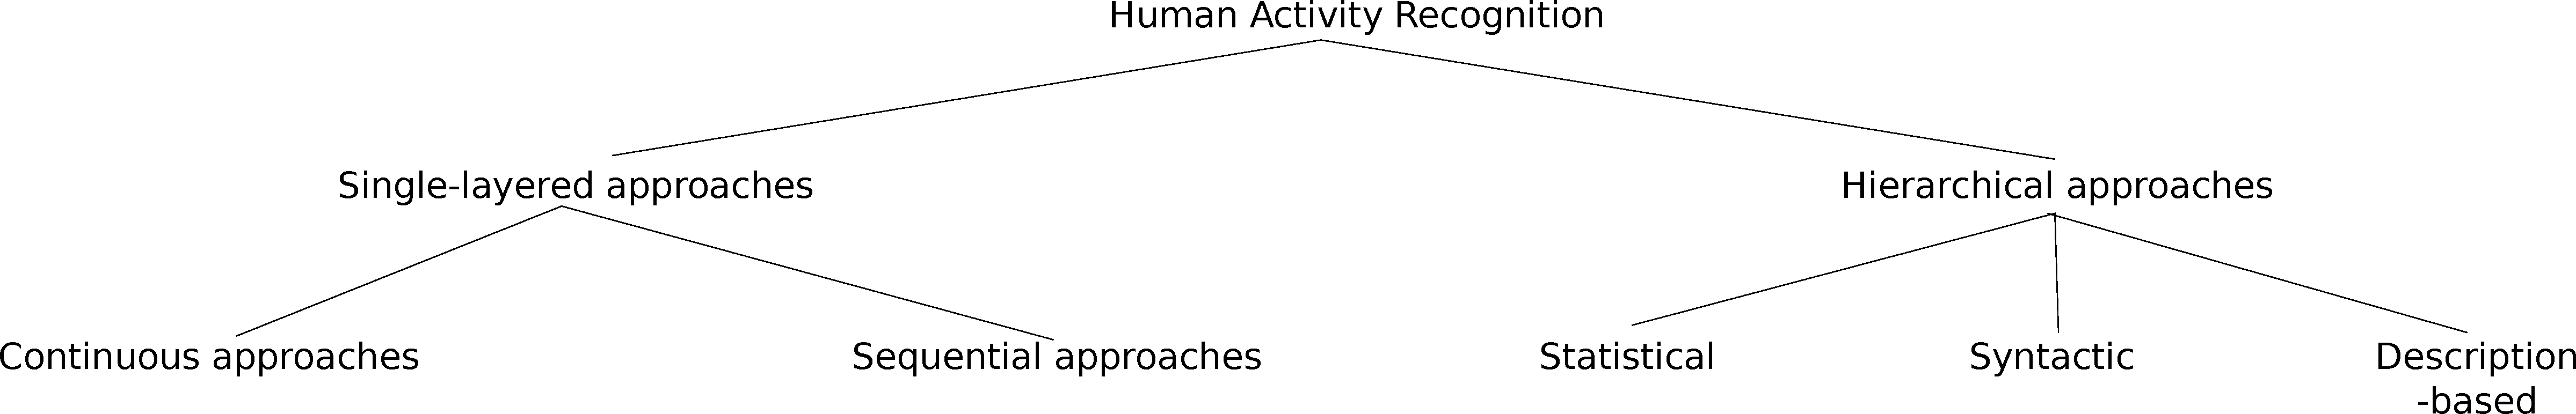
\includegraphics[width=\textwidth]{fig/img_Aggarwal_Taxonomy2.pdf}
\caption{The taxonomy of research in activity recognition described in \cite{Aggarwal11_HumanActivity}.}
\label{fig:taxonomy}
\end{figure}

\subsection{Single-layered approaches}
They represent activities in terms of raw sensory data\footnote{The original survey \citep{Aggarwal11_HumanActivity} describes single layered approaches as image-based approaches, but it leaves out the systems with other sensing capabilities (e.g. 3D sensors, sonars, GPS, etc.).
However, they can be included too the activities are represented in terms of raw sensory data patterns.}, because of this, the activity descriptions are trained from datasets.

%Sensory data is processed to obtain particular descriptive features of the scene which are compared with known activity patterns. 
%These patterns can be obtained in a supervised or unsupervised fashion (e.g. common occurrences of a specific action). 
%Most of them are based in computer vision and machine learning techniques.

Single-layered approaches are suitable to recognize short-term and simple activities as gestures, movements of the body or simple interactions with objects. 
This is mainly because the amount of sensory data grows very easily and long-term activities would require to process larger amounts of data. 
Also, because activities are not always performed in the same way, even by the same individual; the shorter the activity, the more accuracy that will be attained.
An finally, because they are dependant on the sensors and on the environmental conditions (e.g. lighting, point of view).


\subsubsection{Continuous approaches\footnote{`Space-time approaches' in \citep{Aggarwal11_HumanActivity}}} % BEFORE: Space-Time approaches

The activities are recognized by analysing continuous sensory data and compare it with an activity pattern.

An activity is represented as a block of data along time where the activity was performed, and it is considered as a whole.
A volume (or hyper-volume) is built by concatenating the sensor readings in time.
The dimension of the data will depend on the sensing capabilities of the system; for example, a video stream would require 3 dimensions $(X,Y,T)$ and a RGBD camera would be able to use 4 dimensions $(X,Y,Z,T)$, etc. %TODO Consider RGB values..., what happens with other dimensions, e.g. temperature?
The sensory input is compared with the activity patterns to measure similarity.
If a threshold is fulfilled, then the activity is labelled.

The advantages of this approach is that it is relatively fast and doesn't require domain knowledge. 
However, it is very dependant of the sensory input, the continuity of the data, how the activity is performed and of the point of view where the scene is being observed. %TODO HOMEWORK: What about interpolating the data in incomplete situations.

There are many examples of this approach.
In \citep{Bobick2001_RecHuMovTemp} a video stream of aerobics exercises was analysed by attaching to every pixel a vector indicating the presence and recency of motion. 
Then the stream was compared online with previously described activities to look for matching. 
In \citep{Ke2007_SpTmpShapeAR}, volumes were built by attaching similar regions of adjacent frames.
Then, the problem was transformed in an object matching problem by comparing the shapes of the volumes (sensory stream and activity patterns).

\subsubsection{Sequential approaches} %TODO Go deeper.

Sequential approaches represent activities as a sequence of states. 
A state is a vector of features observed in the scene in a specific time.
Finally, the sequence is analysed depending on the activity representation.
There are two approaches: exemplar-based and model-based.

In exemplar-based approaches, activities, or a class of them, are represented as a sequence of states. 
Then the sensory input is compared in similarity with the patterns.
An example can be found in \citep{Darrell1993_STGestures}, where states are built from view models.
Templates of activities are from sequences of states associated with a physical change (e.g. rotation and scale).
The dynamics of articulated objects in scene were recognized using the dynamic time warping algorithm (DTW) to the sequence of states.

In model based approaches, the sequence of states is compared with a set of probabilistic models of activities. The models are built assuming a temporal dependence between the states, so the transitions are modelled probabilistically using hidden Markov models (HMM) or dynamic bayesian networks (DBN).

The first work to use HMM to recognize activities was \citep{Yamato1992_RecHA_HMM}. They transformed a video stream into a sequence of vectors of image features. Then every vector was transformed to a symbol using vector quantization. Finally, a set of HMMs were created to model the activities, and their parameters were optimized. 


%TODO %TODO %TODO %TODO %TODO %TODO %TODO %TODO %TODO %TODO %TODO %TODO %TODO %TODO %TODO %TODO 
%TODO %TODO %TODO %TODO %TODO %TODO %TODO %TODO %TODO %TODO %TODO %TODO %TODO %TODO %TODO %TODO 

\subsection{Hierarchical approaches}
Hierarchical approaches for activity recognition refer to those where complex activities are represented in terms of simpler ones. 
Multiple layers are defined to represent activities in different levels of complexity.
Low level activities can be recognized using single-layered approaches. 

Hierarchical approaches are also adequate to represent activities symbolically by using the multi-layered organization to describe semantic relations.
By these means, hierarchical approaches are less dependant to training data and they can integrate domain knowledge more easily.

Hierarchical approaches can be categorized, regarding the applied methodology for recognition as statistical, syntactical and description-based. %TODO Expand.


\subsubsection{Statistical}
They are based in the hierarchical construction of statistical state-based models, such as HMMs or DBNs.

First the set of activities to work with is defined and organized hierarchically.
Complex activities are defined in terms of simpler ones and so on until everything can be synthesized to atomic actions.
In this way, many layers are created, from atomic actions to complex activities.
In the bottom level, atomic actions are recognized from sensory data using single-layered sequential approaches. 
As a result, a sequence of feature vectors is transformed into a sequence of atomic actions.
This sequence is the input for the next layer, which now will be treated as a new sequence of observations, and the same approach to recognize atomic actions from the first layer will be applied in the second one, and so on.

In \citep{Oliver2002_LayRepHumActRec}, the authors present layered hidden Markov models (LHMMs) for online activity recognition using data from video, sound and keyboard data. 
They divide their system in three layers: the first one is in charge of recognizing features from every source, the second layer trigger short events from the scene, and the last layer is used for longer activities. 
The hierarchical approach showed an improved performance when compared to single-layered systems.
The training data is used more efficiently and it's more easy to add more detail on specific activities.

Some disadvantages of the statistical approaches is their difficulty to model the temporal structure of events (e.g. $A$ occurred `during'/`before'/`after' $B$) and also, because of their sequential nature, is hard to handle multiple concurrent tasks.

\subsubsection{Syntactic}
In the syntactical approach, activities are represented symbolically as a set of production rules generating a string of atomic actions which is later recognized using parsing techniques.
Atomic actions are obtained with a single-layered approach, however, in higher layers, recognition is performed symbolically.
Context-free grammars (CFGs) and stochastic context-free grammars (SCFGs) are some of the techniques that have been used to recognize high level activities.

One limitation of this approach is the difficulty to handle concurrent activities, and also to consider unexpected events that are not integrated in the grammar.

An example can be found in \citep{Ivanov2000_RecVisActSCFG}.
The authors aim to recognize complex activities in sequences of video.
Two layers are defined; in the lower level, atomic actions are recognized using HMMs, and in the upper one uses SCFGs.
The approach showed to be able to handle longer time activity constraints and more robust to uncertain detections in the lower level.


\subsubsection{Description-based} \label{sec_description_ap}
This approach represent activities as a hierarchy of events, making emphasis in their spatial, temporal and logical structures.

A complex activity is modelled from de occurrence of its sub-events that satisfies certain relations.
The temporal relation between sub-events is also considered in the representation, Allen's calculus is frequently used for this \citep{Allen83_MaintainingKnowledgeTemporal}.
Atomic actions are obtained from sensory data and summarized. %TODO Check out!

Now to recognize activities the problem becomes a \textit{constraint satisfaction problem}, which is NP-hard.
This approach allows a good integration of additional knowledge sources. 
Particularly, the 

There are many possibilities to treat the problem. In \citep{Nevatia2004_OntoVidEvRep,Ryoo2006_RecHuAcCFG}, CFGs are used to represent activities hierarchically, defining temporal relations between sub-events. 
In \citep{Sridhar10_UnsupervisedLearning}, relevant features from the scene are extracted and their behaviour is represented using qualitative spatio-temporal relations (QSTR), then patterns of activities are learnt using Markov chains.



\section{Description-based activity recognition and mobile robotics}

In this project, the selected approach to follow is a description-based one. 
This section presents relevant related work in this line, and in the Answer Set Programming (ASP) paradigm for 
Also, here are presented the precedents of activity recognition with mobile robots.

\subsection{Description-based activity recognition}

As mentioned in section \ref{sec_description_ap}, description-based approaches represent activities hierarchically by decomposing complex activities in sub-events.
The representation should also make emphasis in the spatial, temporal and logical structures.
The recognition is performed by obtaining features from scene (spatial, temporal, logical) and creating a scene description as a \textit{list} of facts, then the problem becomes a constraint satisfaction problem, to find the best activity match for these set of observations. 

\subsubsection{Representation}

%Regarding the representation of activities, there are many desired characteristics. 
An activity is represented as a set of \textit{facts} that needs to be fulfilled with the observations.
This is important, because the facts can be used as logical predicates.
These facts act as constraints between the activity patterns and help to discriminate between them, some of them may be more relevant than the others.

The execution of an activity depends on the subject, and even a particular subject doesn't execute the same activity in the same way.
This is the reason why activities are usually defined in qualitative terms, i.e. in a symbolic more human-like manner.
Quantitative descriptions of activities are still interesting, however, they are restricted to specific domains as rehabilitation or sports.

Regarding the temporal dimension, time can be represented as an instant $t$ or as an interval $(t_1,t_2)$. 
For the instants, simple temporal logic can be used to represent these kind of statements. 
Intervals have been typically treated with two aproaches \citep{Fisher2008_TempRepReas}: Interval temporal logics \citep{Moszkowski1983_RDC} and Allen's interval algebra \citep{Allen83_MaintainingKnowledgeTemporal}.

%Interval temporal logics have been typically used in the description of computer, particularly hardware and protocols.
%TODO EXPAND Check the article by Allen

Allen's interval algebra was introduced as a calculus for temporal reasoning.
It defines 13 possible relations between intervals, and provides a composition table that can be used for reasoning about temporal descriptions of events.

Qualitative spatial representations are the focus of study of Qualitative Spatial Representations (QSR).
These are a set of calculi which allow a machine to represent and reason about spatial entities \citep{Cohn2008_QSRR}, e.g. lines, dots, regions, etc.
They are usually combined with a temporal representation (e.g. Allen's interval algebra) to represent behaviour dynamics.

%Tony Cohn
In \citep{Sridhar10_PhD_UnsupervisedLearningEvent}, activities are learnt, in an unsupervised fashion, and recognized from video sequences by reasoning under qualitative spatio-temporal representations (QSTR). 
Objects positions and their trajectories are extracted from scenes and represented in QSTR.
Activities are learnt using a Markov Chain Monte Carlo (MCMC) procedure to find the maximum a posteriori probability (MAP) of candidate interpretations.
This work shows an example of unsupervised learning of activities, using simulated and real examples.
The qualitative approach (QSTR) is robust to changes in the execution of actions and to sensory errors.
Finally, the categorization of activities showed to be reliable in learning functional object categories which provides semantic information from the scene.
On the other hand, some limitations of this work are a fixed point of view and a posterior analysis.
The analysis is performed only in short video sequences, and in short activities.
The search space grows very easily as the scene becomes more complex.

%Jay Young
In \citep{Young13_PredcitingSituatedBehaviour,Young14_EffectsTraining}, QSTR are applied to the analysis of multi-agent behaviour in the RoboCup simulation league, particularly in estimating future behaviours. 
Positions, trajectories and orientation of the agents in scene are represented using region connection calculus (RCC), qualitative trajectory calculus (QTC) and the Star calculus respectively. 
Other agent's behaviours are learnt by using a HMM, which is fed with the current observations and a window of previous ones. 
As not all the data is relevant, this is first filtered. 
This work presents a study of activity prediction.
The results show that qualitative representations are more easy to treat general cases of activities and require less training data. 
Some drawbacks are that the system posses global information from the environment, and the domain is restricted.

In


\subsubsection{Reasoning}

% Mohan & JL Wyatt
% Shiqui Zhang

% Alessandro Saffiotti 
% (Cirillo, Pecora, Coradeschi)

% Siskind
% Event recognition

% Henry Kautz


\subsection{Mobile robotics}
While a large A robot is an ideal system to perform 

% Michael Karg
% Dondrup (lincoln)
% Group at TUM
% Karinne Ramirez
% RoboEarth




% Aggarwal

\section{Answer Set Programming} % Because is one of the main contributions, I put it appart.
% Group of Viena - Thomas Eiter
% Group of Texas Tech
% Group of Turkey
% Group at ASU

\subsection{ASP Solvers}
% DVL
% ROSoClingo





% 1.5 ACTIVITY RECOGNITION WITH A MOBILE ROBOT
%A robot can be roughly conceived as a physical entity capable of sensing and performing actions in the world.
%With this in mind, it seems clear that a robot, with sufficient sensing capabilities, is a good candidate to perform the task.

%\subsection{ASP}

% 2 - ANSWER SET PROGRAMMING
% General background
% Related work to AR


% 3 - ASP + Robots -> ROSoClingo
% 
%================================================
%================================================
%================================================

